\documentclass{article}%
\usepackage[T1]{fontenc}%
\usepackage[utf8]{inputenc}%
\usepackage{lmodern}%
\usepackage{textcomp}%
\usepackage{lastpage}%
\usepackage{geometry}%
\usepackage{graphicx}%
\usepackage{tikz}%
\usepackage{pgfplots}%
%
\title{Simply Supported Beam Engineering Report}%
\author{mylatexfossee}%
\date{\today}%
%
\begin{document}%
\normalsize%
\maketitle%
\tableofcontents%
\newpage%
\section{Introduction}%
\label{sec:Introduction}%
Engineering report generated automatically using Python + PyLaTeX.

%
\section{Beam Description}%
\label{sec:BeamDescription}%


\begin{figure}[h!]%
\includegraphics[width=0.8\linewidth]{fossee_assets/simply_supported_beam.png}%
\end{figure}

%
\section{Data Source}%
\label{sec:DataSource}%
Force values are read directly from the provided Excel file.

%
\section{Input Data}%
\label{sec:InputData}%
\begin{tabular}{|c|c|c|}%
\hline%
x&Shear Force&Bending Moment\\%
\hline%
0.0&45.0&0.0\\%
\hline%
1.5&36.0&60.75\\%
\hline%
3.0&27.0&108.0\\%
\hline%
4.5&18.0&141.75\\%
\hline%
6.0&9.0&162.0\\%
\hline%
7.5&0.0&168.75\\%
\hline%
9.0&{-}9.0&162.0\\%
\hline%
10.5&{-}18.0&141.75\\%
\hline%
12.0&27.0&108.0\\%
\hline%
13.5&{-}36.0&60.75\\%
\hline%
15.0&{-}45.0&0.0\\%
\hline%
\end{tabular}

%
\section{Shear Force Diagram}%
\label{sec:ShearForceDiagram}%

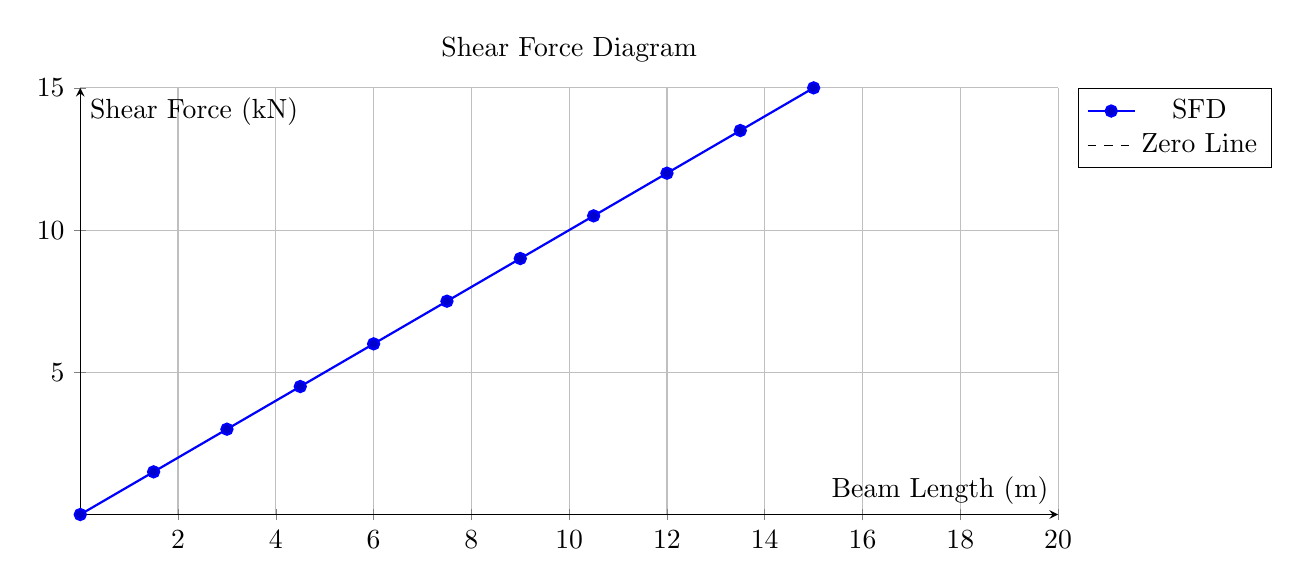
\begin{tikzpicture}
\begin{axis}[
width=14cm,
height=7cm,
grid=both,
xlabel={Beam Length (m)},
ylabel={Shear Force (kN)},
title={Shear Force Diagram},
legend style={at={(1.02,1)},anchor=north west},
axis lines=middle
]
\addplot+[thick,mark=*] coordinates {(0.0,0.0) (1.5,1.5) (3.0,3.0) (4.5,4.5) (6.0,6.0) (7.5,7.5) (9.0,9.0) (10.5,10.5) (12.0,12.0) (13.5,13.5) (15.0,15.0)};
\addplot[dashed] coordinates {(0,0) (20,0)};
\legend{SFD,Zero Line}
\end{axis}
\end{tikzpicture}

%
\section{Bending Moment Diagram}%
\label{sec:BendingMomentDiagram}%

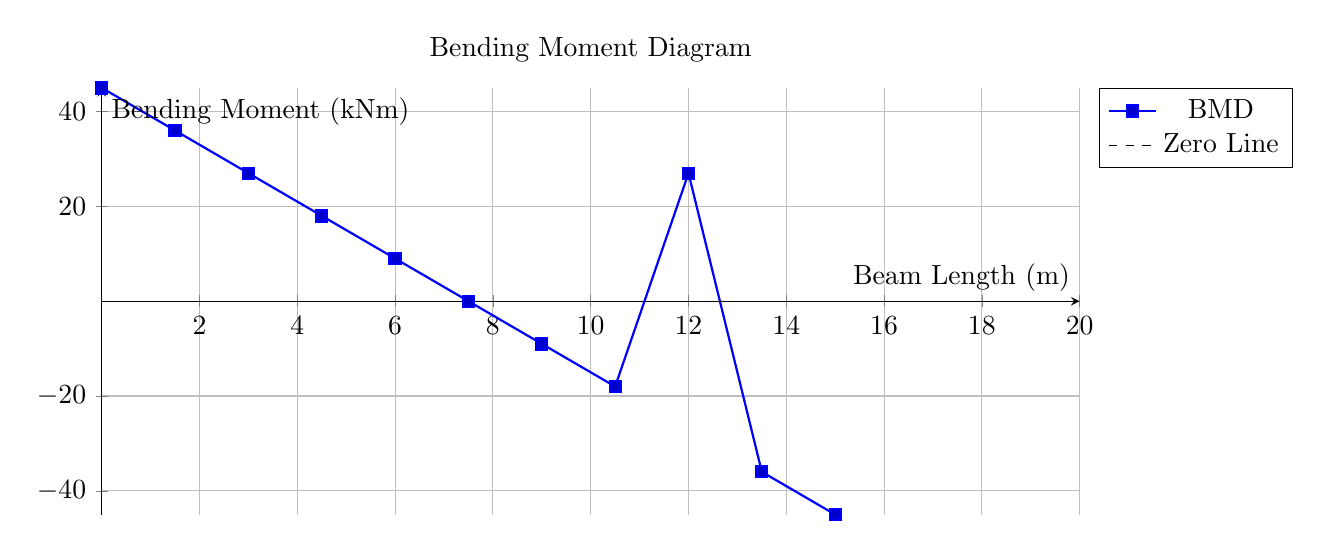
\begin{tikzpicture}
\begin{axis}[
width=14cm,
height=7cm,
grid=both,
xlabel={Beam Length (m)},
ylabel={Bending Moment (kNm)},
title={Bending Moment Diagram},
legend style={at={(1.02,1)},anchor=north west},
axis lines=middle
]
\addplot+[thick,mark=square*] coordinates {(0.0,45) (1.5,36) (3.0,27) (4.5,18) (6.0,9) (7.5,0) (9.0,-9) (10.5,-18) (12.0,27) (13.5,-36) (15.0,-45)};
\addplot[dashed] coordinates {(0,0) (20,0)};
\legend{BMD,Zero Line}
\end{axis}
\end{tikzpicture}

%
\end{document}